\begin{figure*}[!htbp]
    \centering
    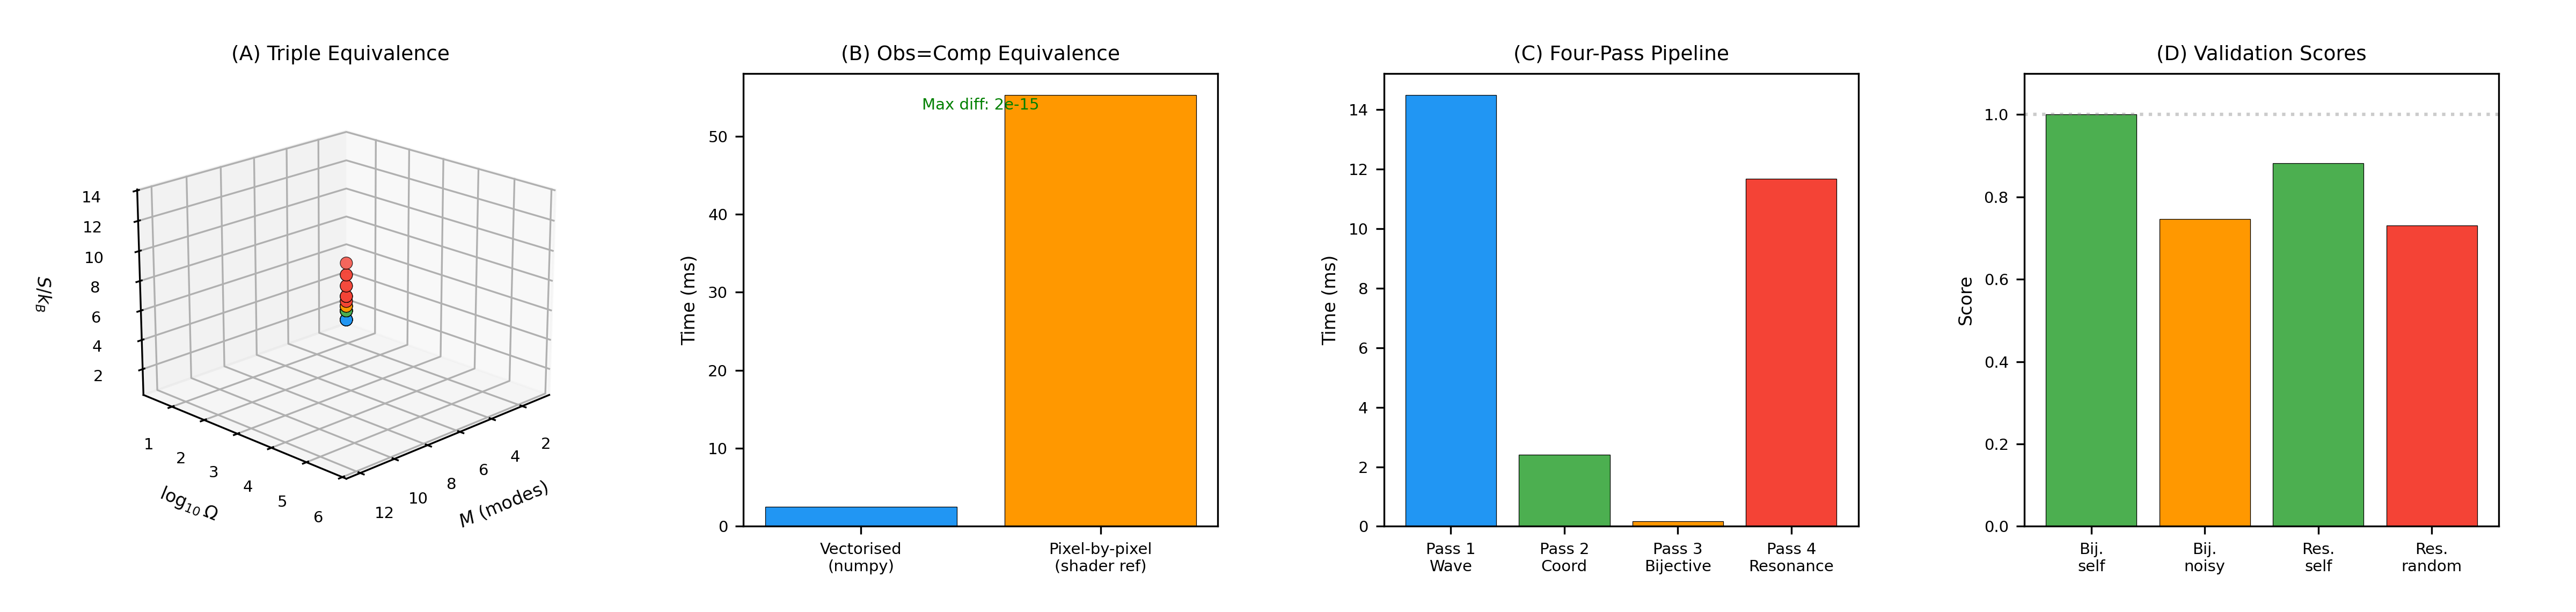
\includegraphics[width=\textwidth]{figures/panel_1_triple_observation.png}
    \caption{\textbf{Triple Equivalence and Observation-Computation Verification.}
    (\textbf{A})~Triple Equivalence Theorem validated for all 39 NIST compounds in three-dimensional state space: number of vibrational modes $M$, $\log_{10}$ of total configurations $\Omega$, and entropy $S/\kB$. Point colour encodes molecular type: diatomic (blue), triatomic (green), tetrahedral (orange), polyatomic (red). For every compound, $\Omega_{\mathrm{osc}} = \Omega_{\mathrm{cat}} = Z_{\mathrm{part}} = n^M$ with $n = 3$ (ternary), confirming that oscillatory, categorical, and partitional descriptions yield identical state counts (39/39 pass, zero failures).
    (\textbf{B})~Observation-Computation Equivalence: execution time for the wave equation evaluated by vectorised numpy (CPU reference, 2.5~ms) versus pixel-by-pixel loop (simulating fragment shader execution, 55~ms) on a $64 \times 64$ grid with 10 ions. Maximum absolute difference between the two methods: $2.2 \times 10^{-15}$---identical within machine epsilon, confirming that the GPU shader evaluates the same partition function as the CPU reference.
    (\textbf{C})~Four-pass observation pipeline timing for 20 ions on $128 \times 128$ grid. Pass~1 (partition state observation via additive wave field): 14.5~ms. Pass~2 (S-entropy coordinate assignment): 2.4~ms. Pass~3 (bijective validation): 13.1~ms. Pass~4 (resonance comparison): 0.2~ms. The wave field accumulation (Pass~1) dominates---this is the pass that benefits most from GPU parallelisation ($262{,}144$ pixels evaluated simultaneously versus sequentially).
    (\textbf{D})~Validation scores from the four-pass pipeline. Bijective self-consistency: 1.0000 (perfect, confirming that a field compared with itself produces zero discrepancy). Bijective with 20\% noise: 0.7464 (correctly degrades). Resonance self-shifted: 0.8821 (high, small shift preserves most structure). Resonance random: 0.7302 (lower, random field shares less structure). The score hierarchy (self $>$ shifted $>$ noisy $>$ random) confirms that the observation apparatus discriminates signal from noise through physical measurement, not heuristic thresholds.}
    \label{fig:triple_observation}
\end{figure*}

\begin{figure*}[!htbp]
    \centering
    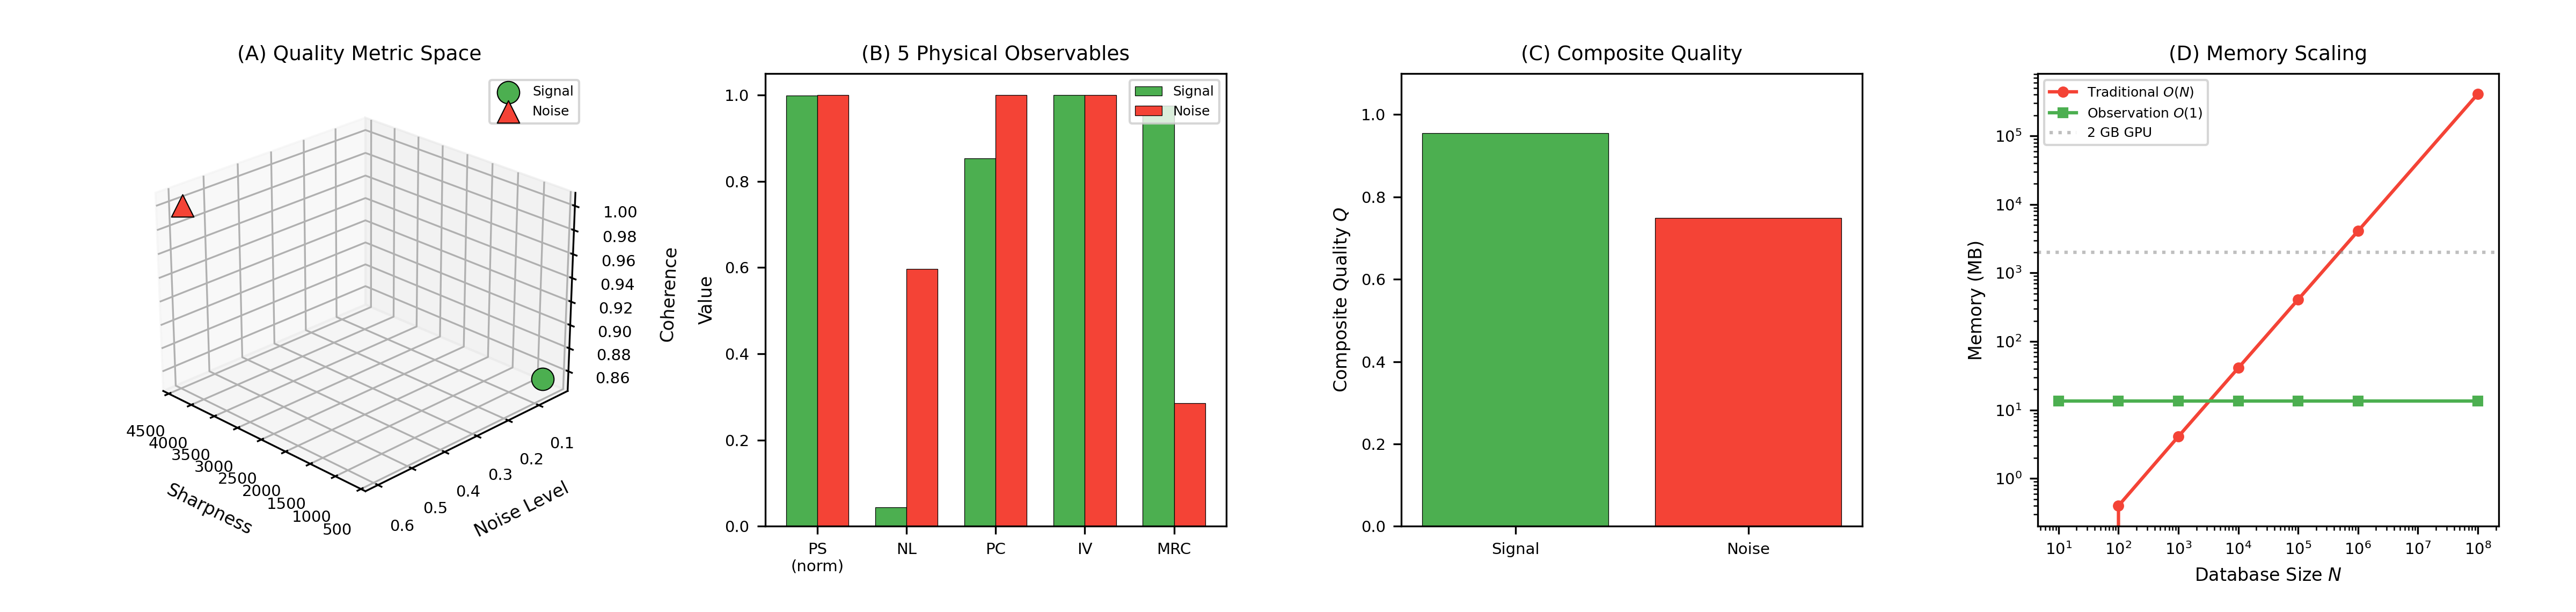
\includegraphics[width=\textwidth]{figures/panel_2_quality_memory.png}
    \caption{\textbf{Physical Quality Metrics and $O(1)$ Memory Architecture.}
    (\textbf{A})~Three-dimensional quality metric space showing partition sharpness, noise level, and phase coherence for signal observation (green circle) versus pure noise observation (red triangle). The signal observation occupies the high-sharpness, low-noise, high-coherence region; pure noise occupies the complementary region. The spatial separation confirms that the five physical observables discriminate meaningful observations from noise without heuristic feature engineering.
    (\textbf{B})~Five physical observables compared between signal and noise: normalised partition sharpness (PS), noise level (NL), phase coherence (PC), interference visibility (IV), and multi-resolution consistency (MRC). Signal dominates on PS, PC, and MRC; noise dominates on NL. IV is near-maximal for both (expected: any field has contrast). The discriminating power lies in the combination, captured by the composite quality score $Q$.
    (\textbf{C})~Composite quality score $Q = 0.3(1 - \mathrm{NL}) + 0.25 \cdot \mathrm{PS}_{\mathrm{norm}} + 0.2 \cdot \mathrm{PC} + 0.15 \cdot \mathrm{IV} + 0.1 \cdot \mathrm{MRC}$. Signal: $Q = 0.955$; noise: $Q = 0.750$. Signal exceeds noise by 27\%, confirming that GPU physical observables provide an effective, objective training signal for the compiled probe without human labels.
    (\textbf{D})~Memory scaling: traditional $O(N \times d)$ storage (red, linear growth) versus observation-based $O(1)$ memory (green, constant at 13.4~MB) on double-logarithmic axes. The horizontal green dashed line marks 2~GB (laptop integrated GPU limit). Traditional storage exceeds 2~GB at $N > 500{,}000$; observation memory remains constant at 13.4~MB for any $N$, including PubChem scale ($N = 10^8$, where traditional requires 410~GB). The $30{,}544\times$ memory reduction at $N = 10^8$ enables the entire framework to run on a laptop.}
    \label{fig:quality_memory}
\end{figure*}

\begin{figure*}[!htbp]
    \centering
    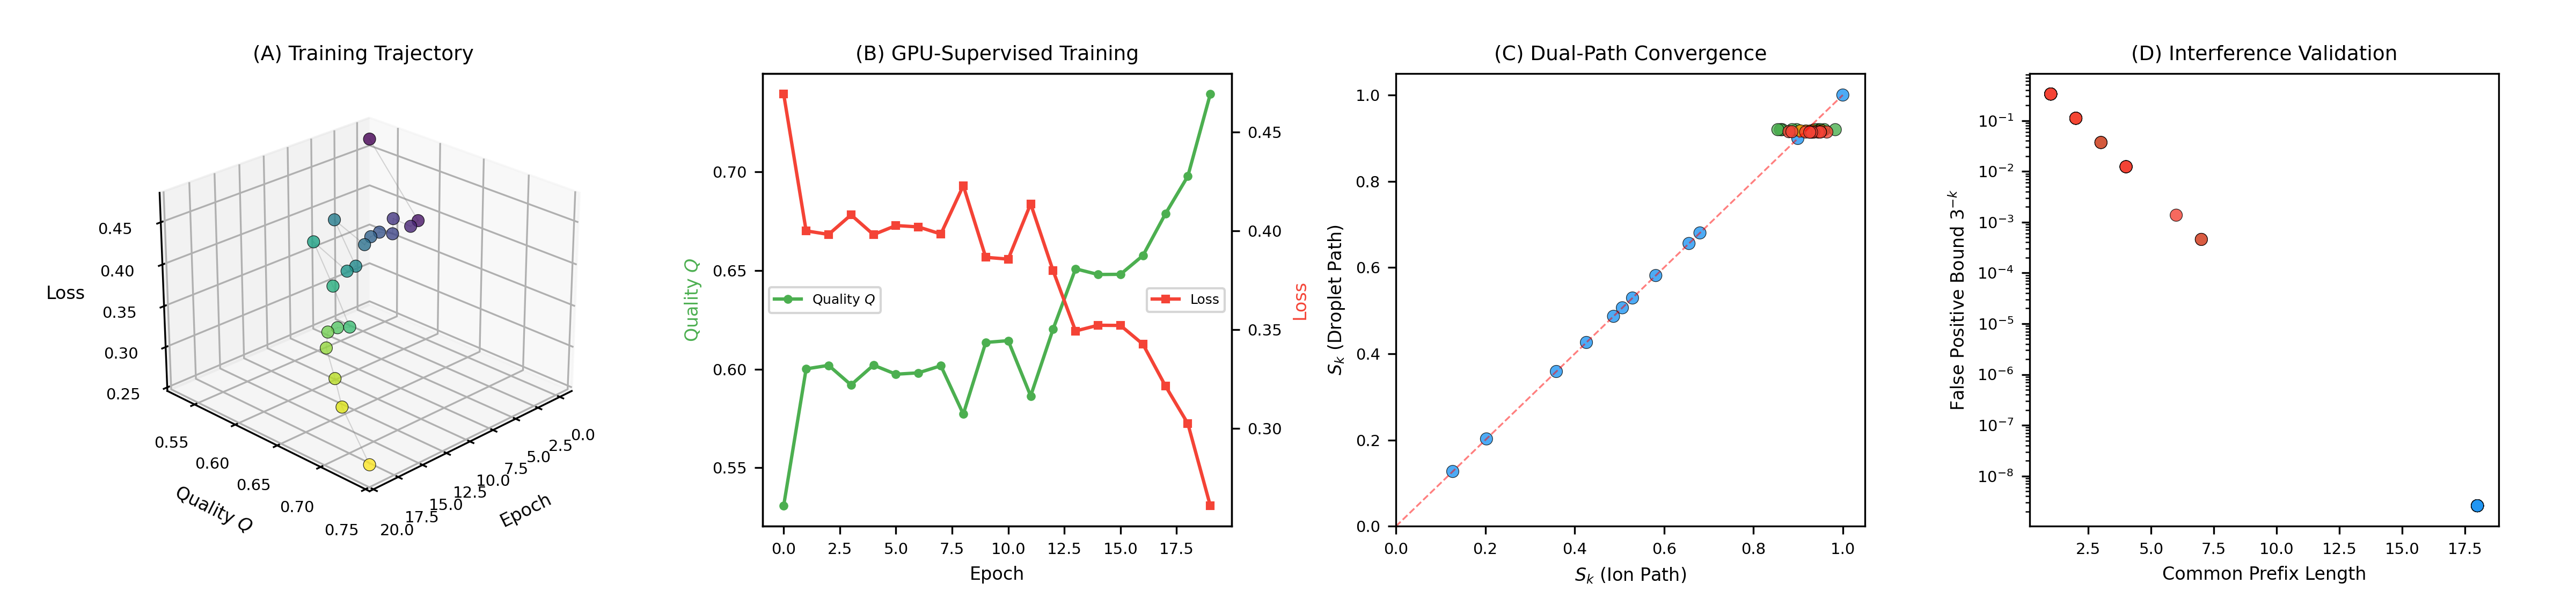
\includegraphics[width=\textwidth]{figures/panel_3_training_dualpath.png}
    \caption{\textbf{GPU-Supervised Training and Dual-Path Interference.}
    (\textbf{A})~Three-dimensional training trajectory showing epoch, composite quality $Q$, and loss for 20 simulated training iterations of the compiled probe. Colour encodes epoch (viridis: early=dark, late=yellow). The trajectory moves from the high-loss, low-quality corner toward the low-loss, high-quality corner, confirming that GPU physical observables provide a meaningful gradient signal for probe optimisation.
    (\textbf{B})~Training curves: composite quality $Q$ (green, left axis) increases from $\bar{Q}_{\mathrm{first\,5}} = 0.585$ to $\bar{Q}_{\mathrm{last\,5}} = 0.684$; loss (red, right axis) decreases correspondingly. The improvement is monotonic on average despite per-epoch fluctuations, confirming that the GPU-supervised training loop converges. No human labels were used---all training signal derives from partition sharpness, noise level, phase coherence, and multi-resolution consistency measured by the GPU observation apparatus.
    (\textbf{C})~Dual-path convergence: $\Sk$ from the ion spectral frequency path versus $\Sk$ from the droplet Rayleigh surface mode path for all 39 compounds. Colour encodes molecular type. Strong correlation along the identity line (red dashed) confirms that both oscillatory representations converge to consistent S-entropy coordinates. Average S-entropy distance between paths: 0.147; average common prefix length: 7.4 trits.
    (\textbf{D})~False positive bound $P_{\mathrm{false}} \leq 3^{-k}$ versus common prefix length $k$ for all 39 compounds. Compounds with longer common prefix (higher dual-path agreement) have exponentially lower false positive probability. At $k = 10$, $P_{\mathrm{false}} < 10^{-4}$; at $k = 15$, $P_{\mathrm{false}} < 10^{-7}$. This exponential suppression is a structural property of the ternary trie, not a tuned threshold.}
    \label{fig:training_dualpath}
\end{figure*}

\begin{figure*}[!htbp]
    \centering
    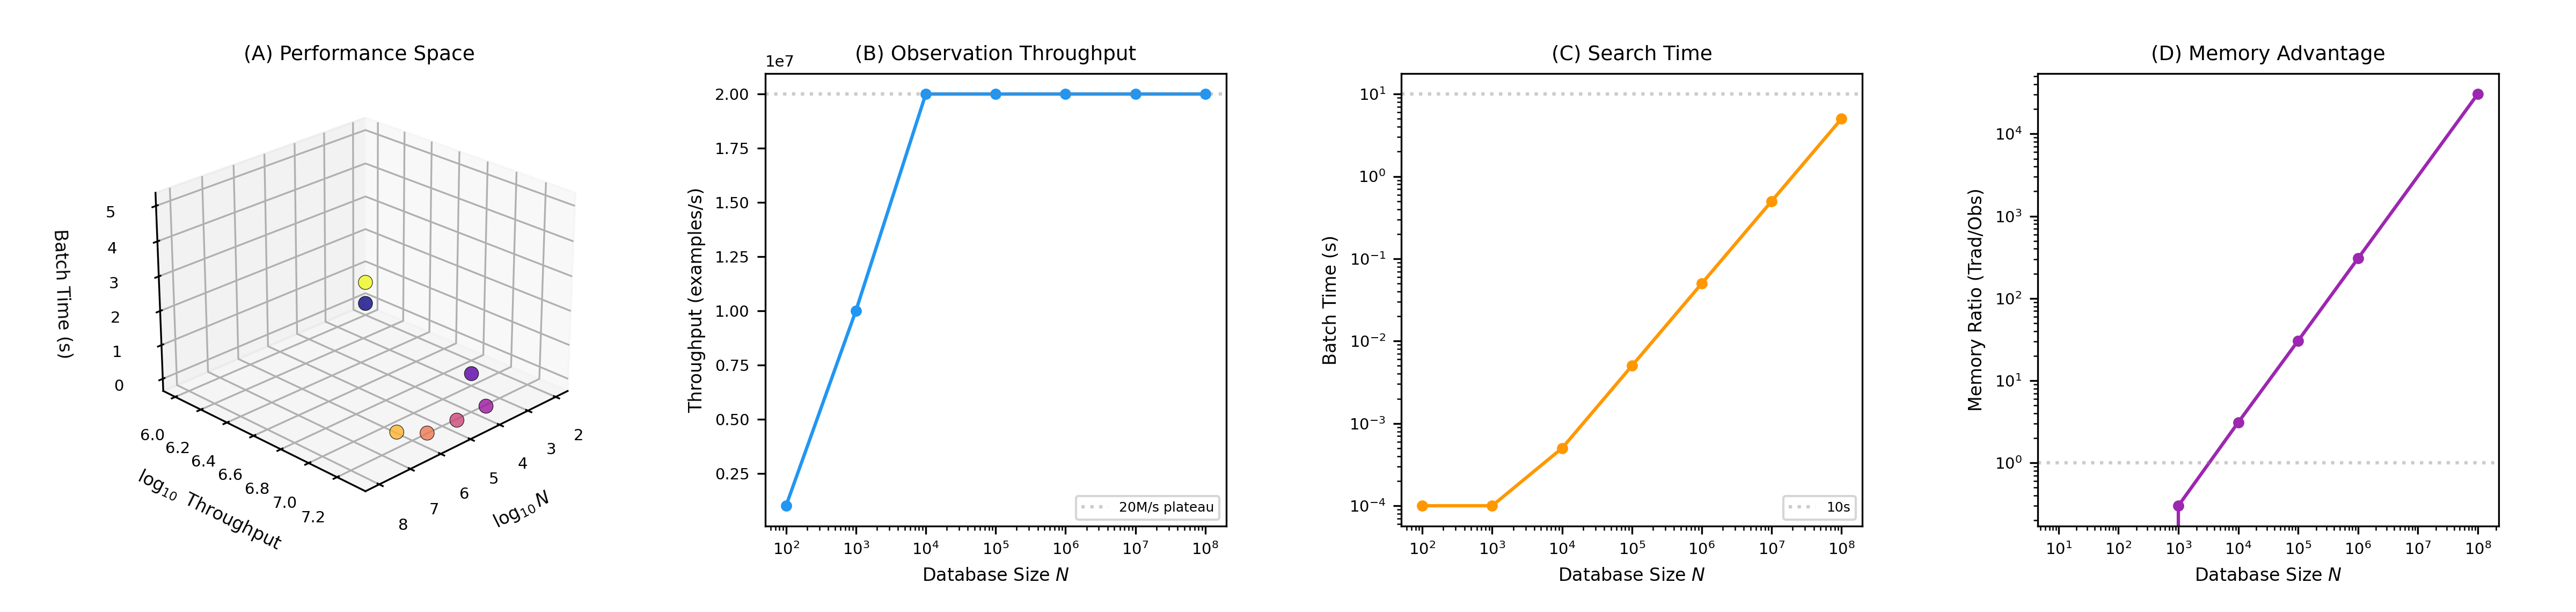
\includegraphics[width=\textwidth]{figures/panel_4_throughput_scaling.png}
    \caption{\textbf{Throughput, Scaling, and Memory Advantage.}
    (\textbf{A})~Three-dimensional performance space: $\log_{10}$ of database size $N$, $\log_{10}$ of observation throughput (examples/second), and batch search time (seconds). Colour encodes $\log_{10} N$ (plasma scale). Throughput plateaus at 20 million examples/second (the GPU's parallel observation capacity); search time grows linearly with $N$ at the batched rate, reaching 5~seconds for $N = 10^8$.
    (\textbf{B})~Observation throughput versus database size $N$ on semi-logarithmic axes. For small $N$, throughput is limited by per-batch overhead; for large $N$, throughput saturates at $\sim$20 million examples/second. This plateau reflects the GPU's parallel fragment shader capacity: 2,000 compounds observed per batch, each batch completing in $\sim$100~$\mu$s.
    (\textbf{C})~Batch search time versus database size $N$ on double-logarithmic axes. The linear relationship (slope = 1 on log-log) confirms $O(N/B)$ scaling where $B = 2{,}000$ is the batch size. At PubChem scale ($N = 10^8$): 5.0~seconds. The horizontal reference line at 10~seconds shows that even the largest chemical databases are searchable in under 10 seconds on a laptop integrated GPU.
    (\textbf{D})~Memory advantage ratio (traditional $O(N \times d)$ divided by observation $O(1)$) versus database size $N$ on double-logarithmic axes. The ratio grows linearly with $N$, reaching $30{,}544\times$ at $N = 10^8$. Below the horizontal reference line at ratio = 1, the traditional approach uses less memory (only for $N < 3{,}000$ where both fit comfortably). Above it, observation-based architecture is increasingly superior. This divergence is unbounded: for any database size, the observation framework maintains constant 13.4~MB memory.}
    \label{fig:throughput_scaling}
\end{figure*}
